\section{Analyse}
	Als Gesamtübersicht und als Eruierungshilfe der einzelnen Teilprobleme wurde zu Beginn der Lösungsfindung eine Skizze entworfen. Diese beinhaltet alle nötigen Elemente des Produkts und stellt diese in Relation zueinander dar. Produkt-Komponenten wurden dabei in blau, externe in grün dargestellt.
	
	\begin{figure}[h!]
		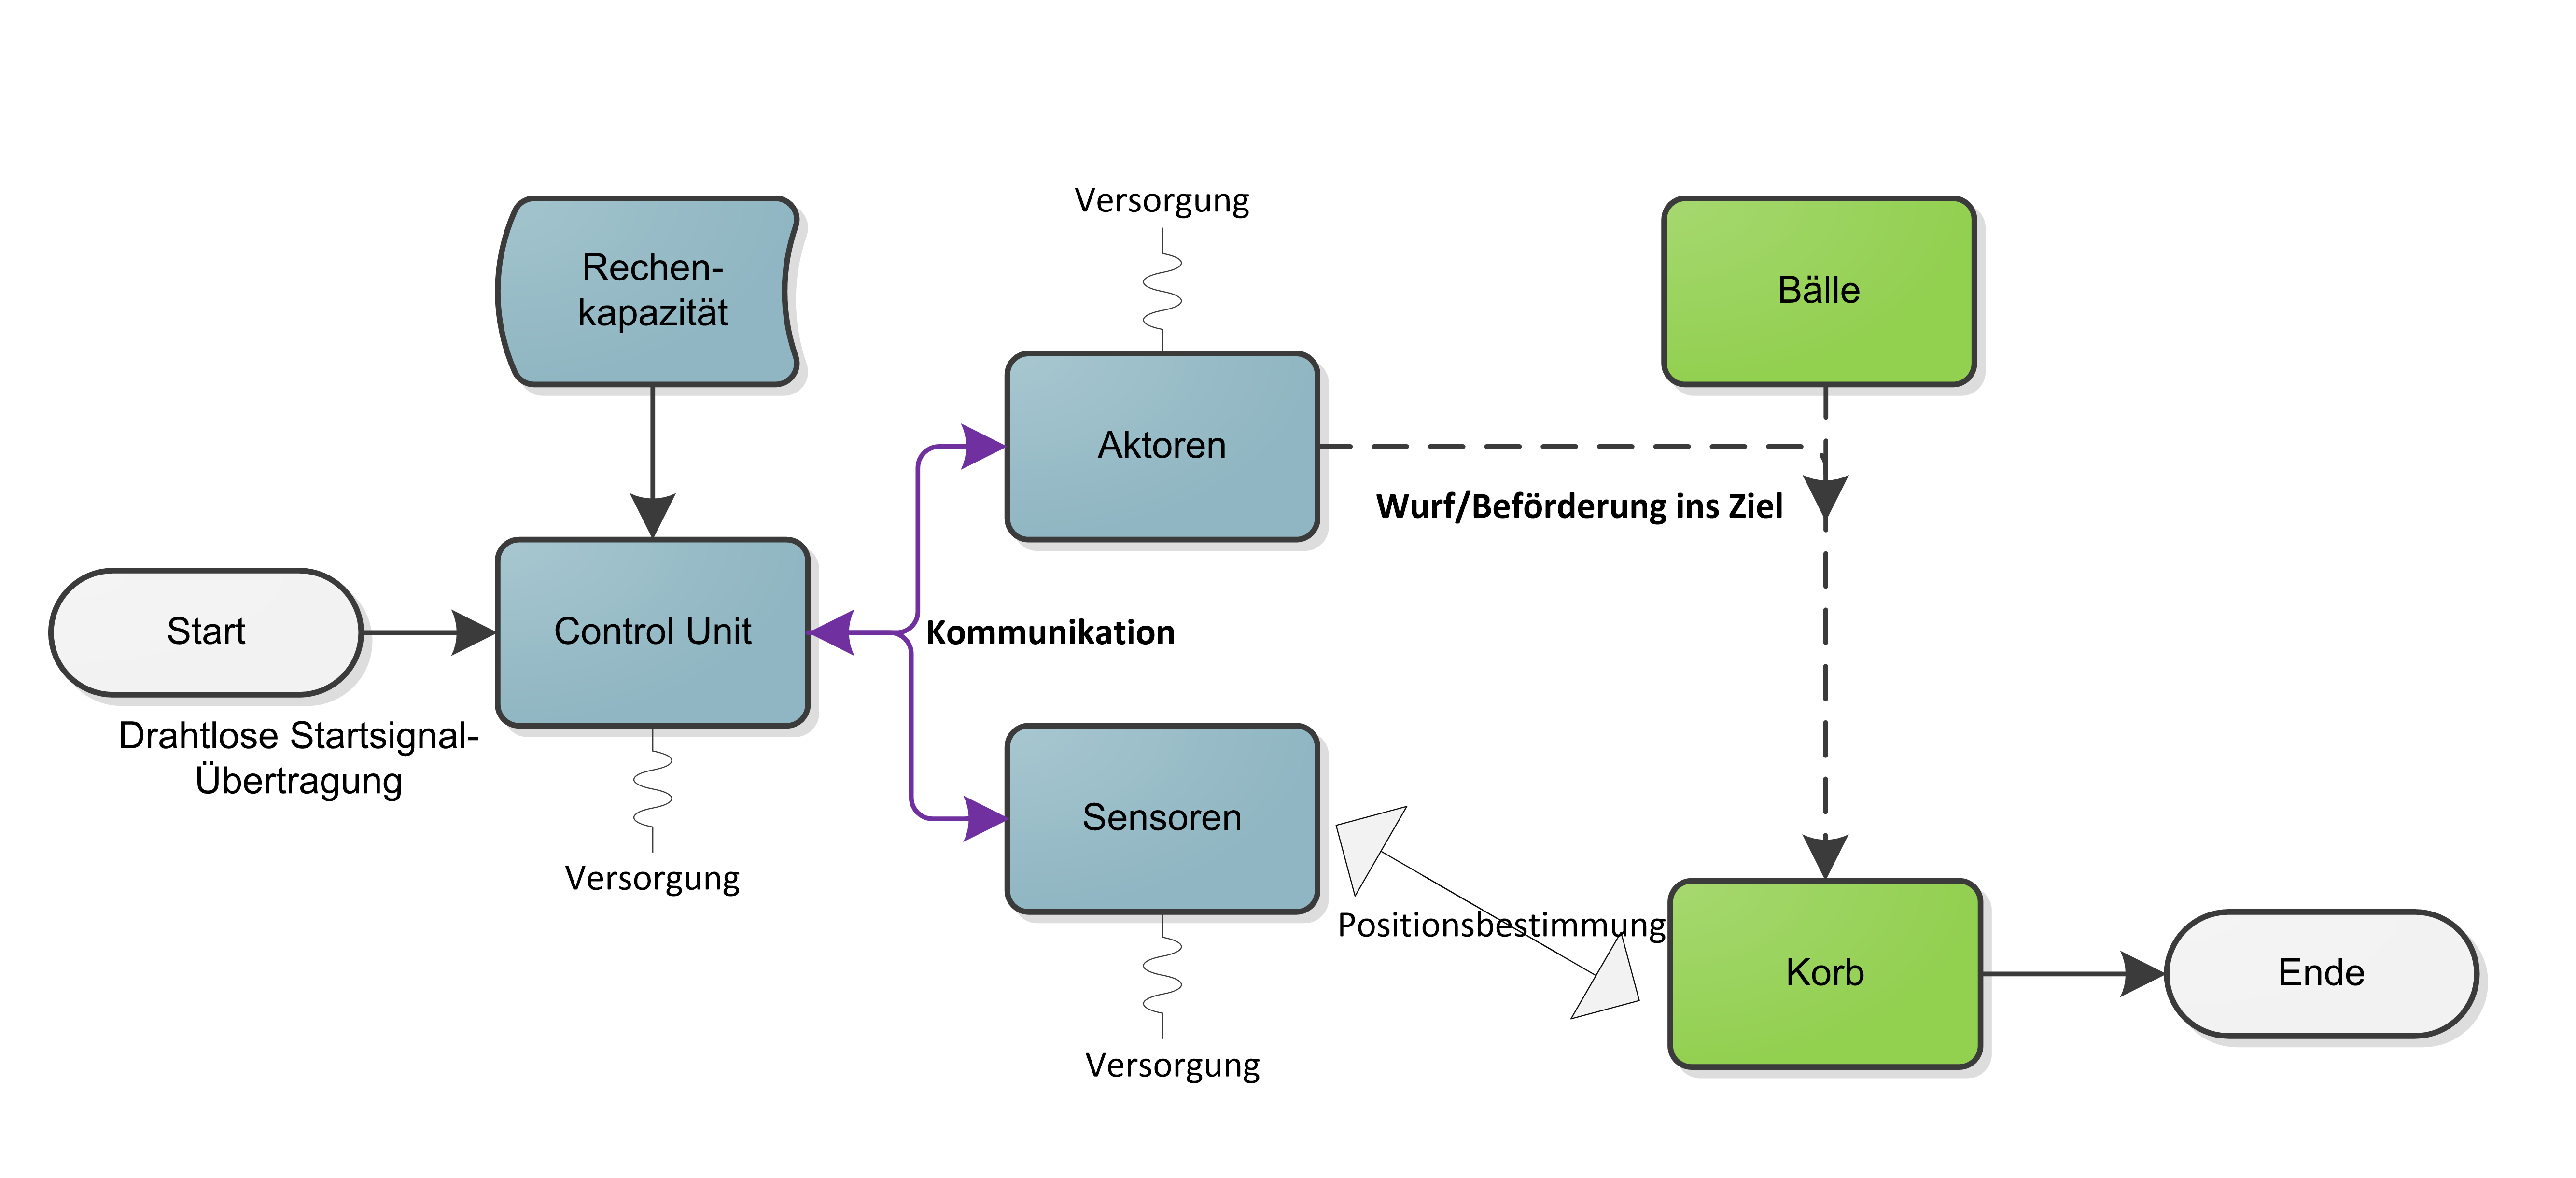
\includegraphics[width=1.1\textwidth]{Morphologie/Bilder/Blockschaltbild}
		\centering
		\caption{Funktionsskizze zur Aufgabenstellung}
		\label{abb:Blockschaltbild} 
	\end{figure}
	
	Aus der Abbildung \ref{abb:Blockschaltbild} ergeben sich folgende Teilprobleme:
	\begin{itemize}
		\item Startgerät / Endgerät
		\item Startbefehlsübermittlung (drahtlos)
		\item Rechenkapazität (immer inklusive Verteileinheit)
		\item Versorgung der Steuerung / Sensoren
		\item Sensorik (Korberkennung)
		\item Ausgangslage der Bälle
		\item Weg des Balles (zum Korb)
	\end{itemize}
	Als nächster Schritt werden die Teilprobleme genauer definiert. Der Technologierecherche entspringende Lösungsansätze sollen die Problembereiche möglichst gut abdecken.
	
	\subsection{Beurteilung der Teilprobleme}
		Durch die Definition von passenden Beurteilungskriterien sollen die verschiedenen Lösungsansätze für ein Teilproblem taxiert werden. An dieser Stelle bieten sich die definierten Ziele der Teamcharta an:
		
		\begin{enumerate}
			\item Treffgenauigkeit
			\item Geschwindigkeit
			\item Gewicht
		\end{enumerate}		
		Da diese Ziele direkt durch die Eigenschaften des Werfers definiert werden, sollen sie auch direkt in die Auswahl der Komponenten miteinfliessen. Um das Kriterium Treffergenauigkeit auf alle Teilprobleme abbilden zu können, wurde dieses Ziel als Zuverlässigkeit neu definiert. Nachfolgend der Pool von Bewertungskriterien, aus welchem anschliessend für jedes Teilproblem ein geeignetes Set zur Bewertung ausgewählt wurde.
		
		\begin{enumerate}
			\item Zuverlässigkeit
			\item Geschwindigkeit
			\item Gewicht
			\item Kosten
			\item Aufwand
		\end{enumerate}		
		Der Faktor Zuverlässigkeit erhält in jedem Teilproblem einen hohen Wert. Der Aufwand belegt in der Regel einen kleinen Faktor, da er in einem Schulprojekt einen sekundären Stellenwert hat. Der Faktor der Kosten wurde bewusst im Mittelfeld angesiedelt, um den Fokus auf die Zielsetzung zu legen, aber trotzdem teuren Produkten ein Nachteil einzuhandeln.
		In der Regel ist die Verteilung der Punkte pro Kriterium so geregelt, dass die am schlechtesten geeignete Lösung 1 Punkt erhält, die beste Lösung 5 Punkte und die restlichen einen Wert dazwischen.\\
		\\
		Um die nachfolgende Beschreibung zu den Kriterien richtig zu interpretieren, ist die Beurteilung in Anhang \ref{apx:BeurteilungTeilprobleme} zusätzlich zum jeweiligen beschreibenden Text hinzuzuziehen. 
		
		\subsubsection{Startgerät – Endgerät}
			\textit{Ist zusammen mit Anhang \ref{apx:StartgeraetEndgeraet} zu betrachten.}
			\begin{itemize}
				\item Zuverlässigkeit\\
				Ein Notebook beruht auf langjährigen, gut dokumentierten und erprobten Technologien (drahtlos Kommunikation, sowie dazugehöriger Software). Ein Taster hingegen muss neu gebaut werden, kann daher fehleranfällig sein.
				\item Kosten\\
				Das Smartphone/Notebook wird von einem Teammitglied zur Verfügung gestellt. Ein Taster müsste neu gebaut oder eingekauft werden.
				\item Kompatibilität\\
				Ein Smartphone besitzt nur ein Betriebssystem mit beschränkter Funktionalität. Mit einem Notebook kann man viele verschiedene Software-Lösungen erstellen.
				\item Aufwand\\
				Das Smartphone/Notebook wird von einem Teammitglied zur Verfügung gestellt, es entsteht vor allem softwaretechnischer Aufwand. Für einen Taster müsste ein eigenes kleines System entwickelt werden.
			\end{itemize}
			
		\subsubsection{Startbefehlsübermittlung}
			\textit{Ist zusammen mit Anhang \ref{apx:Startbefehluebermittlung} zu betrachten.}
			\begin{itemize}
				\item Zuverlässigkeit\\
				Bluetooth (und WLAN) basieren auf wohlbekannten, gut dokumentierten, standardisierten Technologien. Akustische Signale, sowie Infrarot sind hingegen eher störanfällig.
				\item Kosten\\
				Bluetooth (und WLAN) sind Teil der eingebauten Technologie in einem modernen Smartphone / Notebook. Für Infrarot und Akustischen Signalen müssten entsprechende Instrumente angeschafft werden.
				\item Aufwand\\
				Da jedes Teammitglied sowohl ein Smartphone, als auch einen Laptop mit WLAN/Bluetooth besitzt, wäre hier der Aufwand minimal. Das Auswerten eines Akustischen Signals ist hingegen aufwändig, fehleranfällig und benötigt zusätzliche Elektronik.
			\end{itemize}	
			
		\subsubsection{Rechenkapazität}
			\textit{Ist zusammen mit Anhang \ref{apx:Rechenkapazitaet} zu betrachten.}
			\begin{itemize}
				\item Zuverlässigkeit\\
				Smartphone und Embedded Prozessoren sind sehr zuverlässig, da sie on-board sind. Ein Notebook als externe Recheneinheit ist aufgrund der dafür benötigten Datenverbindung fehleranfällig.
				\item Geschwindigkeit\\
				Embedded Prozessoren sind für genau eine spezifische Aufgabe ausgelegt und dimensioniert. Ein Notebook als Recheneinheit ist aufgrund der Datenübermittlung fehleranfällig und tendenziell langsamer.
			 	\item Gewicht\\
			 	Embedded Prozessoren sind für genau eine spezifische Aufgabe ausgelegt und dimensioniert und beinhalten nur das absolut Notwendige. In einem Smartphone sind viele Module verbaut, von denen zur Aufgabenerfüllung eigentlich nur wenige gebraucht werden, was sich negativ auf das Gesamtgewicht auswirkt.
				\item Kosten\\
				Das Smartphone/Notebook wird von einem Teammitglied zur Verfügung gestellt. Ein eingebetteter Prozessor müsste zugekauft werden.
				\item Aufwand\\
				Für einen Embedded Prozessor müsste eine eigene Stromversorgung, drahtlos-Kommunikations-Modul, etc. gebaut werden. Ein Notebook beruht auf wohlbekannten, gut dokumentierten Technologien.
			\end{itemize}
			Zusätzliche Erläuterung: Es wird davon ausgegangen, dass ein Embedded Prozessor günstiger Bauart eingesetzt würde.
			
		\subsubsection{Sensorik}
			\textit{Ist zusammen mit Anhang \ref{apx:Sensorik} zu betrachten.}
			\begin{itemize}
				\item Geschwindigkeit\\
				Eine Foto mit einer Smartphone Kamera ist schnell geschossen und kann direkt im Smartphone bearbeitet werden. Ein Laser muss viele Punkte abscannen und dabei mechanisch geschwenkt werden.
				\item Genauigkeit\\
				Ein Laser misst viele Punkte, kann daher ein sehr detailliertes Abbild schaffen. Ultraschallmessungen hingegen eher unpräzise.  
				\item Zuverlässigkeit\\
				Laservermessungen sind dank des detaillierten Abbilds zuverlässig in der Korberkennung. Infrarot ist aufgrund des vielen Fremdeinflusses (bsp. Lichtstrahler an Spielfeldrand) unzuverlässig.
				\item Kosten\\
				Das Smartphone mit integrierter Kamera wird von einem Teammitglied zur Verfügung gestellt. Für einen Laser muss aufgrund der mechanischen Justierung zusätzliche Bauteile eingekauft werden.
				\item Aufwand\\
				Für die Objekterkennung mit Kamera gibt es bereits meherere bekannte Frameworks, was den Aufwand drastisch minimieren würde. Auf der anderen Seite muss bei Verwendung eines Lasers aufgrund der benötigten mechanischen Justierung zusätzlichen Aufwand betrieben werden.
			\end{itemize}
			
		\subsubsection{Versorgung Steuerung / Sensorik}
			\textit{Ist zusammen mit Anhang \ref{apx:VersorgungSteuerungSensorik} zu betrachten.}
			\begin{itemize}
				\item Zuverlässigkeit\\
				Ein Akku hat im Vergleich zu einem Netzteil höhere Spannungsschwankungen.
				\item Gewicht\\
				(hier als Vorteil, da als Ballast anrechenbar) Akku kann zur Gewichtsbestimmung entfernt werden.
				\item Kosten\\
				Netzteile sind günstig und alte Netzteile können für diese Aufgabe recycelt werden. Akkus müssten neu gekauft werden.
				\item Aufwand\\
				Netzteile können in kompletter Form gekauft werden. Akku’s müssen mit Elektronik stabilisiert und geregelt werden.
			\end{itemize}	
		
		\subsubsection{Ausgangslage der Bälle}
			\textit{Ist zusammen mit Anhang \ref{apx:AusgangslageDerBaelle} zu betrachten.}
			\begin{itemize}
				\item Geschwindigkeit\\
				Alle Bälle in einem Behälter braucht wenig Zeit, ist daher die beste Lösung. Der Drehkranz ist schwerfällig und langsam.
				\item Gewicht\\
				Der Trichter ist eine einfache, minimalistische Konstruktion, die wenig Gewicht aufweist. Der Drehkranz ist gegenteilig eine grosse, schwere Konstruktion mit mehreren Aktoren.
				\item Zuverlässigkeit\\
				Die Bälle in einem Trichter können schnell verstopfen. Ein sauber konstruiertes und aufgebautes Magazin ist sehr zuverlässig. 
				\item Kosten\\
				Der Trichter hat eine einfache, minimalistische Konstruktion, benötigt daher wenig Material. Der Drehkranz hat viele Aktoren und ein aufwändiges Design.
				\item Aufwand\\
				Die Umsetzung eines Trichters ist einfach und schnell erledigt. Der Drehkranz ist aufwändig.					
			\end{itemize}
			Zusätzliche Erläuterung: Bei der Beförderung der Bälle in einem Behälter wird davon ausgegangen, dass ein wohlgeformte geometrische Figur verwendet wird (bspw. Kugel).
			
			
		\subsubsection{Weg des Balles}
		\textit{Ist zusammen mit Anhang \ref{apx:WegDesBalles} zu betrachten.}\\		
		\enquote{Aus Startposition zu Korb fliegen und abwerfen}, nachfolgend mit (1) bezeichnet.\\	
		\enquote{Aus Startposition, gewinkelt durch Luft werfen}, nachfolgend mit (2) bezeichnet.\\
		\enquote{Aus Startposition, seitlich bewegen, gerade aus durch Luft werfen}, nachfolgend mit (3) bezeichnet.\\
		\enquote{Aus Startpositionmitte gerade zu Begrenzungslinie bewegen und gewinkelt durch Luft werfen}, nachfolgend mit (4) bezeichnet.\\
		\enquote{Aus Startposition zu Begrenzungslinie gerade vor Korb bewegen und durch Luft werfen}, nachfolgend mit (5) bezeichnet.\\	
		
		Nachfolgende Bezeichnungen (..) beziehen sich auf die Nummerierung im Anhang \ref{apx:BeurteilungTeilprobleme}			
			\begin{itemize}
				\item Geschwindigkeit\\
				Je weniger Achsen bewegt werden müssen, desto schneller ist die jeweilige Lösung. (2) muss nur eine Drehbewegung ausführen. (5) muss drei Bewegungen ausführen.
				\item Zuverlässigkeit\\
				Je weniger Achsen bewegt werden müssen, desto zuverlässiger ist die Lösung. (2) muss nur eine Drehbewegung ausführen. (1) muss fliegen und zusätzlich noch ständig nachkorrigieren, äussre Störeinflüsse schwer vorauszusagen.
				\item Genauigkeit\\
				Je mehr Achsen bewegt werden müssen, je mehr Toleranzen, Fehler und Justierungen treten ein. (2) hat nur eine bewegliche Achse. (1) und (5) haben viele bewegliche Achsen und viele unbekannte Störeinflüsse.
				\item Gewicht\\
				Je mehr Achsen bewegt werden müssen, je mehr Antriebe, Materialien und Elektronik wird benötigt. (2) ist stationär. (4) und (5) haben viele bewegliche Achsen. 
				\item Kosten\\
				Je mehr Achsen bewegt werden müssen, je teurerer werden die jeweiligen Ausführungen. (2) ist stationär. (4) und (5) haben viele bewegliche Achsen. (1) kann zudem im Testfall abstürzen und so teure Teile zerstören.
				\item Aufwand\\
				(1) softwaretechnischer Aufwand ist immens. (2) stationäre Lösung im Vergleich eher einfach zu realisieren. (4) und (5) haben viele bewegliche Achsen, jede zusätzliche Achse erfordert weiteren Aufwand.	
			\end{itemize}

